A deficiency in the prior approach is that each word has only one embedding. The \textbf{polysemy} (same word, different meanings / contexts) are ignored. In order to tackle polysemy, I need to find embedding methods that assign multiple embeddings to a single word. This is known as \textbf{Multi Sense Embeddings}, and Apoorv pointed me to \cite{neelakantan2015efficient} for a state of the art multi sense word embedding model.

Before I discuss that model, it is useful to review the Skip-gram with negative sampling model used by Word2Vec since the multi sense embedding model is an extension of the original skipgram model.

\subsection{Background on Skip-gram with Negative Sampling}

The Skip-gram model assumes that words have contexts based on the words around them, and do not have contexts with words that are far away from them. This is known as the distributional hypothesis. In the skipgram model, $v(w_{i, x}) \in R^d$ is the vector representation of the word $w_{i, x}$ for $i \in 1 ... n$ where $n$ is the number of words in the corpus, and $C_x$ is the corpus. $d$ is the dimensionality of the embedding. Given a pair of words $(w_{i, x}, c)$, the probability that the word $c$ (for context) is observed in the context of word $w_{i, x}$ is given by

\[ P(D = 1 | v(w_{i, x}), v(c)) = \frac{1}{1+\exp{-v(w_{i, x})^n v(c)}}\]

The probability of not observing the word $c$ in the context of $w_{i, x}$ is given by

\[ P(D = 0 | v(w_{i, x}), v(c)) = 1 - P(D = 1 | v(w_{i, x}), v(c)) = 1 - \frac{1}{1+\exp{-v(w_{i, x})^n v(c)}}\]

Give na training set containing the sequence of words $w_{1, x}, w_{2,x} ... w_{n, x}$, the word embeddings are learned by maximizing the objective function:

\begin{align*}
J(\theta) = &\sum_{(w_{i, x}, c_{i, x}) \in G^+} \sum_{c \in c_{i, x}} \log{P(D=1 | v(w_{i,x}), v(c)})\\
&+ \sum_{(w_{i, x}, c_{i, x}) \in G^-} \sum_{c' \in c'_{i, x}} \log{P(D=0 | v(w_{i,x}), v(c')})
\end{align*}

where $w_{i, x}$ is the $i$th word in the training corpus $C_x$, $c_{i, x}$ is the set of observed context words of word $w_{i, x}$ and $c'_{i, x}$ is the set of randomly selected noisy context words for the word $w_{i, x}$. $G^+$ consists of the set of all observed word-context pairs $(w_{i, x}, c_{i, x})$ where $i \in 1 ... n$. $G^-$ consists of the pairs $(w_{i,x}, c'_{i, x})$ where $i \in 1 ... n$ where $c'_{i, x}$ is the set of randomly selected noisy context words for the word $w_{i, x}$.

For each training word $w_{i, x}$ the set of context words $c_{i, x} = \{ w_{i - R_i, x} ... w_{i - 1, x} w_{i + 1, x} ... w_{i + R_i, x} \}$ which includes $R_i$ words to the left and right of the given word. $R_i$ is the window size considered for the word $w_{i,x}$ uniformly randomly sampled from the set $1 ... W$ where $W$ is the maximum context window size.

The set of noisy context words $c'_{i, x}$ is constructed by randomly sampling $S$ noisy context words for each word in the context $c_{i, x}$. The noisy context words are randomly sampled from the following distribution:

\[P(w_{i, x}) = \frac{P_{unigram}(w_{i,x})^\frac{3}{4}}{Z}\]

where $P_{unigram}(w_{i,x})$ is the unigram distribution of the words and $Z$ is the normalization constant.

\subsection{Multi Sense Skipgram Model}

\cite{neelakantan2015efficient} extended the skip-gram model by letting each \textbf{sense} of word have its own embedding.

\begin{quote}
(We) let each sense of word have its own embed- ding, and induce the senses by clustering the em- beddings of the context words around each token. The vector representation of the context is the average of its context words’ vectors. For every word type, we maintain clusters of its contexts and the sense of a word token is predicted as the cluster that is closest to its context representation. After predicting the sense of a word token, we perform a gradient update on the embedding of that sense. The crucial difference from previous approaches is that word sense discrimination and learning em- beddings are performed jointly by predicting the sense of the word using the current parameter estimates.\footnote{\cite{neelakantan2015efficient}}
\end{quote}

In the extended model, each word $w_{i,x}$ is associated with a global vector $v_g(w_{i,x})$ and each sense of the word has an embedding $v_s(w_{i,x}, k)$ for $k \in 1 ... K$ where $K$ is the number of senses of the word. Each sense of the word is also associated with a context cluster with center $\mu(w_{i,x}, k)$ for $k \in 1 ... K$. $K$ and the dimension of the vectors $d$ are hyperparameters.

Let's say I have a word $w_{i,x}$. The context of that word is $c_{i, x} = \{w_{i-R_i, x} ... w_{i-1, x} w_{i+1, x} ... w_{i+R_i,x}\}$ based on the observed context words. The vector representation of the context is defined as the average of the global vector representation of the words in the context. Hence,

\[v_{context}(c_{i,x}) = \frac{1}{2R_i}\sum_{c \in c_{i, x}} v_g(c)\]

\cite{neelakantan2015efficient} used the global vectors of the context words instead of the sense vectors to avoid the computational complexity associated with predicting the sense of the context words. Then, the algorithm predicts $s_{i, x}$, the sense of the word $w_{i,x}$ when associated with the context $c_{i, x}$ using the existing cluster centers of the sense vectors of the word $w_{i,x}$. This portion of the algorithm is similar to the k-means algorithm. The chosen sense $s_{i,x}$ is essentially

\[s_{i,x} = \mathrm{argmax}_{k \in 1 ... K} cossim(\mu(w_{i,x}, k), v_{context}(c_{i,x}))\]

The cluster center is the average of the vector representation of all the contexts which belong to that cluster. $cossim$ is simply the cosine similarity measure used in earlier experiments.

The probability that word $c$ is observed in the context of word $w_{i, x}$ given the sense of word $w_{i,x}$ is

\begin{align*}
&P(D = 1 | s_{i,x}, v_s(w_{i,x}, 1), ... v_s(w_{i,x}, K), v_g(c)) \\
&= P(D=1|v_s(w_{i,x}, s_{i,x}), v_g(c)) \\
&= \frac{1}{1 + e^{-v_s(w_{i,x}, s_{i,x})^n v_g(c)}}
\end{align*}

The probability of not observin the word $c$ in the context of $w_{i,x}$ given the sense of word $w_{i,x}$ is:

\begin{align*}
&P(D = 0 | s_{i,x}, v_s(w_{i,x}, 1), ... v_s(w_{i,x}, K), v_g(c)) \\
&= P(D=0|v_s(w_{i,x}, s_{i,x}), v_g(c)) \\
&= 1 - P(D=1|v_s(w_{i,x}, s_{i,x}), v_g(c)) \\
&= \frac{1}{1 + e^{-v_s(w_{i,x}, s_{i,x})^n v_g(c)}}
\end{align*}

Given a training set containing the sequence of words $w_{1,x}, w_{2,x} ... w_{n,x}$ the word embeddings are learned by maximizing the objective function:

\begin{align*}
J(\theta) = &\sum_{(w_{i,x}, c_{i,x}) \in G^+} \sum_{c \in c_{i,x}} \log P(D = 1 | v_s(w_{i,x}, s_{i,x}), v_g(c)) \\
&+ \sum_{(w_{i,x}, c_{i,x}) \in G^-} \sum_{c' \in c'_{i,x}} \log P(D = 0 | v_s(w_{i,x}, s_{i,x}), v_g(c'))
\end{align*}

The variables $c$ $c'$ $G^+$ and $G^-$ are constructed in the same way as the original Skip-gram with negative sampling model. After predicting the sense of the word, the algorithm updates the embedding of the predicted sense of the word $w_{i,x}(v_s(w_{i,x}, s_{i,x}))$, the global vector of the words in the context and the global vector of the randomly sampled noisy context words. The context cluster center of cluster $s_{i,x}$ for the word $w_{i,x}$, $\mu(w_{i,x}, s_{i,x})$ is updated since context $c_{i,x}$ is updated to the cluster $s_{i,x}$.

By giving each word multiple senses, it disambiguates between different usages of the same word, a limitation that \texttt{word2vec} has as shown in Figure \ref{fig-mssg-demo}.

\begin{figure}[H]
\begin{itemize}
\item Skip-gram: 
\subitem blackberry, macintosh, acorn, pear, plum
\item MSSG:
\subitem pear, honey, pumpkin, potato, nut 
\subitem microsoft, activision, sony, retail, gamestop
\subitem macintosh, pc, ibm, iigs, chipsets
\end{itemize}
\caption{Words similar to the word ``apple''. Each sublist represents a different sense of the word ``apple''. For the original skip-gram model, only one sense is available. However, using the Multi-Sense Skipgram (MSSG) model, I am able to disambiguate between different senses of the word ``apple''}
\label{fig-mssg-demo}
\end{figure}

This is useful in the codeword detection problem. However, before tackling that, I wanted to ensure that the code runs first. A good trial run would be to test this code (which \cite{neelakantan2015efficient} provides at \url{https://bitbucket.org/jeevan_shankar/multi-sense-skipgram/overview} on the Reddit corpus to detect multiple senses of words.

Trying to compile this project using the given \texttt{make\_cp.sh} produces the following errors:

\begin{lstlisting}
(default)➜  multi-sense-skipgram git:(master) sh make_cp.sh
error: error while loading CharSequence, class file '/Library/Java/JavaVirtualMachines/jdk1.8.0_31.jdk/Contents/Home/jre/lib/rt.jar(java/lang/CharSequence.class)' is broken
(class java.lang.RuntimeException/bad constant pool tag 18 at byte 10)
error: error while loading Comparator, class file '/Library/Java/JavaVirtualMachines/jdk1.8.0_31.jdk/Contents/Home/jre/lib/rt.jar(java/util/Comparator.class)' is broken
(class java.lang.RuntimeException/bad constant pool tag 18 at byte 20)
error: error while loading AnnotatedElement, class file '/Library/Java/JavaVirtualMachines/jdk1.8.0_31.jdk/Contents/Home/jre/lib/rt.jar(java/lang/reflect/AnnotatedElement.class)' is broken
(class java.lang.RuntimeException/bad constant pool tag 18 at byte 76)
error: error while loading Arrays, class file '/Library/Java/JavaVirtualMachines/jdk1.8.0_31.jdk/Contents/Home/jre/lib/rt.jar(java/util/Arrays.class)' is broken
(class java.lang.RuntimeException/bad constant pool tag 18 at byte 765)
/var/folders/sw/0j_h3wdj6zjcpkyty1gw_rj00000gq/T/sbt_994f79e2/API.scala:424: error: java.util.Comparator does not take type parameters
	private[this] val sortClasses = new Comparator[Symbol] {
                                            ^
5 errors found
\end{lstlisting}

Turns out this can be resolved by uncommenting the line \lstinline{<useManifestOnlyJar>false</useManifestOnlyJar} in \texttt{pom.xml} for the code. Running the demo bash script would run NP-MSSG on the \texttt{text8} corpus.

\subsection{Modifying the MSSG Algorithm to Solve Community Problem}

In the codeword detection problem, we are interested in finding how different communities use the same words. For example, if ``cheeseburger'' was used by one single community to denote financial fraud while the rest of the communities use it to denote the food, the MSSG algorithm will tell us that there are two senses of the word ``cheeseburger''. However, to use this directly to solve this problem, I needed to modify the MSSG algorithm to tell me \textbf{how different communities utilize the different senses of the words}.

The key to the word sense association is $s_{i,x} = \mathrm{argmax}_{k \in 1 ... K} cossim(\mu(w_{i,x}, k), v_{context}(c_{i,x}))$ In other words, the sense chosen for a word encountered is the closest cluster center for the word's current average context (a word is associated with multiple cluster centers) in a process very similar to the k-means algorithm.

This process can be exploited to identify the community to which a word sense belongs. For example, let's say that there are 5 communities. Let's also say that ``apple'' has two word senses -- that of the fruit (so it will be associated with words like ``orange'' and ``banana'') and that of the company (so it will be associated with words like ``samsung'' and ``microsoft'').

Let's say that each word sense has an array of frequency counts attached to it that counts the number of times it is chosen as the cluster center in the step $s_{i,x} = \mathrm{argmax}_{k\in 1 ... K} \{sim(\mu(w_{i,x}, k), v_{context}(c_{i,x}))\}$. That means, if in the sentence ``Apple beats Samsung in latest sales.'', ``apple'' is associated the second cluster center, and this sentence appeared in the first community then $count_{\mu(apple, s_{i,x} = 2, community = 1)} += 1$. If in the sentence ``Apple and banana makes a good smoothie.'' is associated with the first cluster center and the sentence comes from the 5th community, then $count_{\mu(apple, s_{i,x} = 1, community = 5)} += 1$.

Then, at the end of training, we should have a histogram, for each word and for each word sense, of the frequency the word is attributed to each community. For example, I may have:

\begin{itemize}
\item For the first sense of the word apple ($s_{i,x} = 1$) in the sense of fruit
\begin{itemize}
\item $count_{\mu(apple, s_{i,x}=1, community=1)} = 5069$
\item $count_{\mu(apple, s_{i,x}=1, community=2)} = 4839$
\item $count_{\mu(apple, s_{i,x}=1, community=3)} = 5143$
\item $count_{\mu(apple, s_{i,x}=1, community=4)} = 3948$
\item $count_{\mu(apple, s_{i,x}=1, community=5)} = 4510$
\end{itemize}
\item For the first sense of the word apple ($s_{i,x} = 2$) in the sense of the company
\begin{itemize}
\item $count_{\mu(apple, s_{i,x}=2, community=1)} = 534$
\item $count_{\mu(apple, s_{i,x}=2, community=2)} = 134$
\item $count_{\mu(apple, s_{i,x}=2, community=3)} = 314$
\item $count_{\mu(apple, s_{i,x}=2, community=4)} = 134$
\item $count_{\mu(apple, s_{i,x}=2, community=5)} = 24506$
\end{itemize}
\end{itemize}

What I may see is that the first sense of the word is pretty evenly distributed across the communities. This means that all the communities are using the word apple in the first sense. However, for the apple company word sense, only the 5th community is using it significantly. This implies that apple as a company is unique in meaning to the 5th community.

This is then directly relevant to codeword detection. A codeword is by definition \textbf{a word that a specific subset of people in an organization (a community) uses differently from others}. Let's say that I were able to identify these communities via a separate method (probably social clustering). Then, given these communities, I would now be able to identify \emph{lingo} that is specific to a community (a subset of the entire organization). Let's say that traders in department x is using the word ``cheeseburger'' to denote an offshore account. Then, the sense of the word ``cheeseburger'' as an offshore account would have high counts for that specific community.

I do note that not only codewords may be detected -- certain communities may simply use words that are unique to their community (e.g. slangs). Nonetheless, these will be interesting in the legal discovery process as well and would be interesting to be identified.

This requires a modification to the NP-MSSG that has a special data structure to label each word with its provenance. This was done in Scala. The output is, along with the original embeddings, a histogram of community counts for each sense of a word $w_{i,x}$.

\begin{landscape}

\begin{figure}[H]
\begin{subfigure}[t]{.3\textwidth}
\centering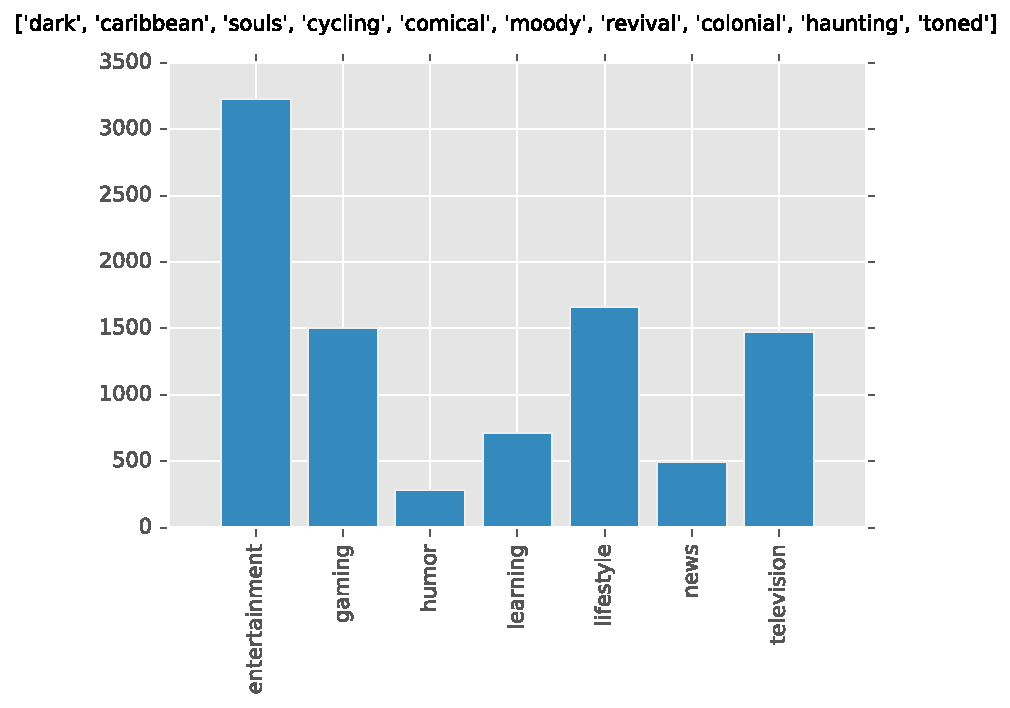
\includegraphics[]{figures/reddit-dark-0.pdf}
\caption{``dark'' sense 1}
\label{fig-reddit-dark-0}
\end{subfigure}
\begin{subfigure}[t]{.3\textwidth}
\centering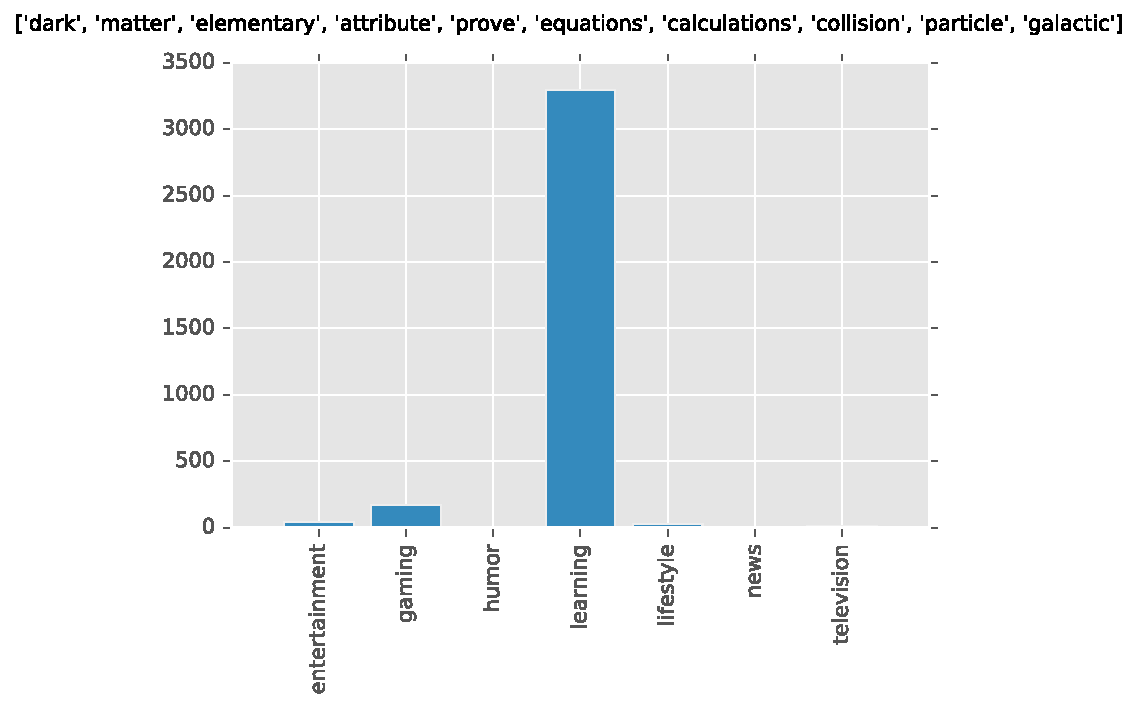
\includegraphics[]{figures/reddit-dark-1.pdf}
\caption{``dark'' sense 2}
\label{fig-reddit-dark-1}
\end{subfigure}
\begin{subfigure}[t]{.3\textwidth}
\centering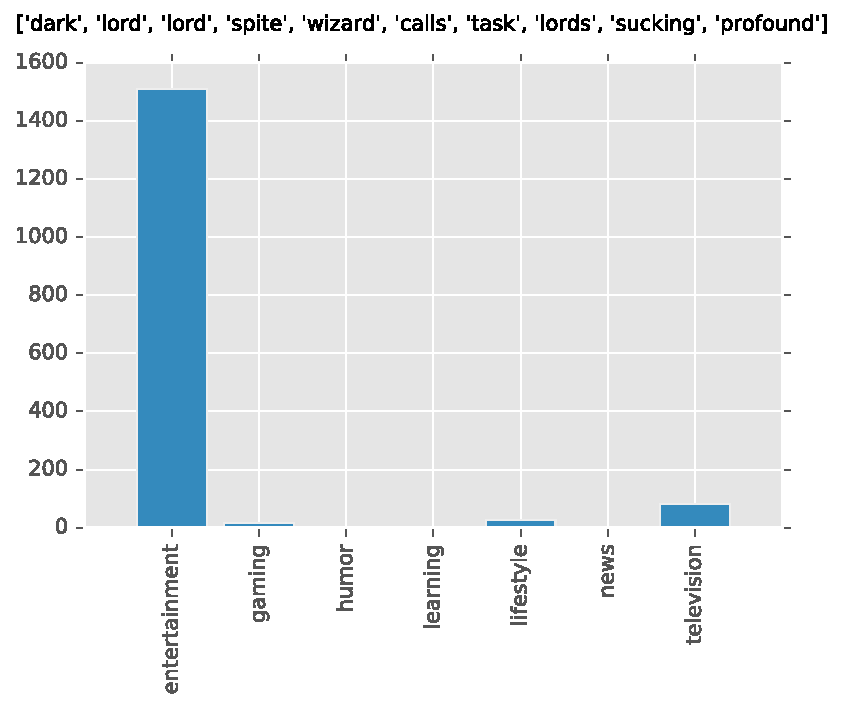
\includegraphics[]{figures/reddit-dark-2.pdf}
\caption{``dark'' sense 3}
\label{fig-reddit-dark-2}
\end{subfigure}
\begin{subfigure}[t]{.3\textwidth}
\centering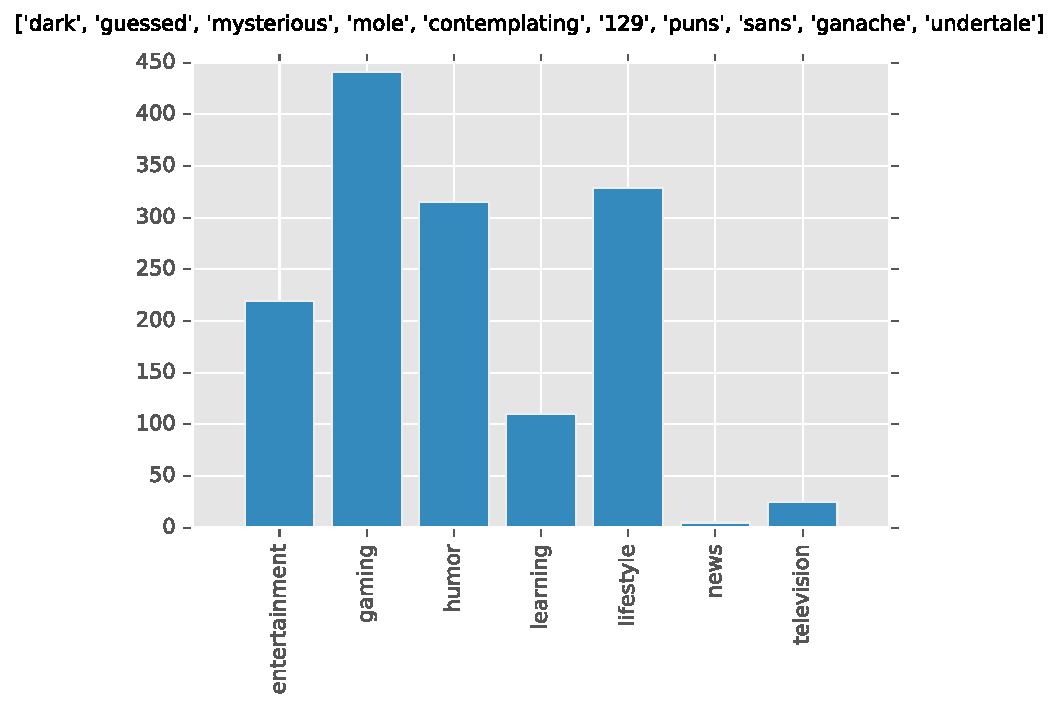
\includegraphics[]{figures/reddit-dark-3.pdf}
\caption{``dark'' sense 4}
\label{fig-reddit-dark-3}
\end{subfigure}
\begin{subfigure}[t]{.3\textwidth}
\centering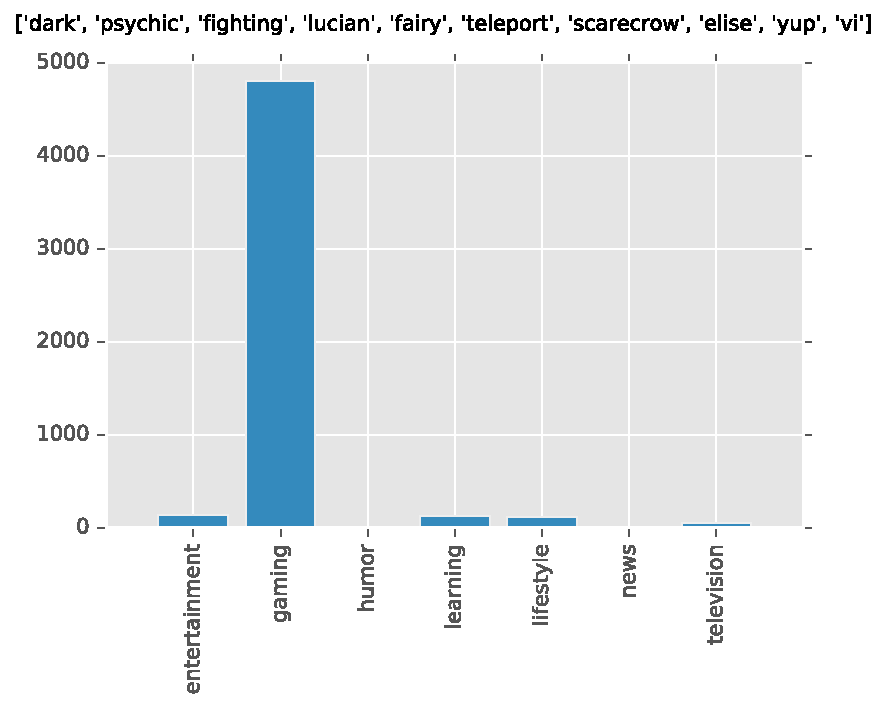
\includegraphics[]{figures/reddit-dark-4.pdf}
\caption{``dark'' sense 5}
\label{fig-reddit-dark-4}
\end{subfigure}
\begin{subfigure}[t]{.3\textwidth}
\centering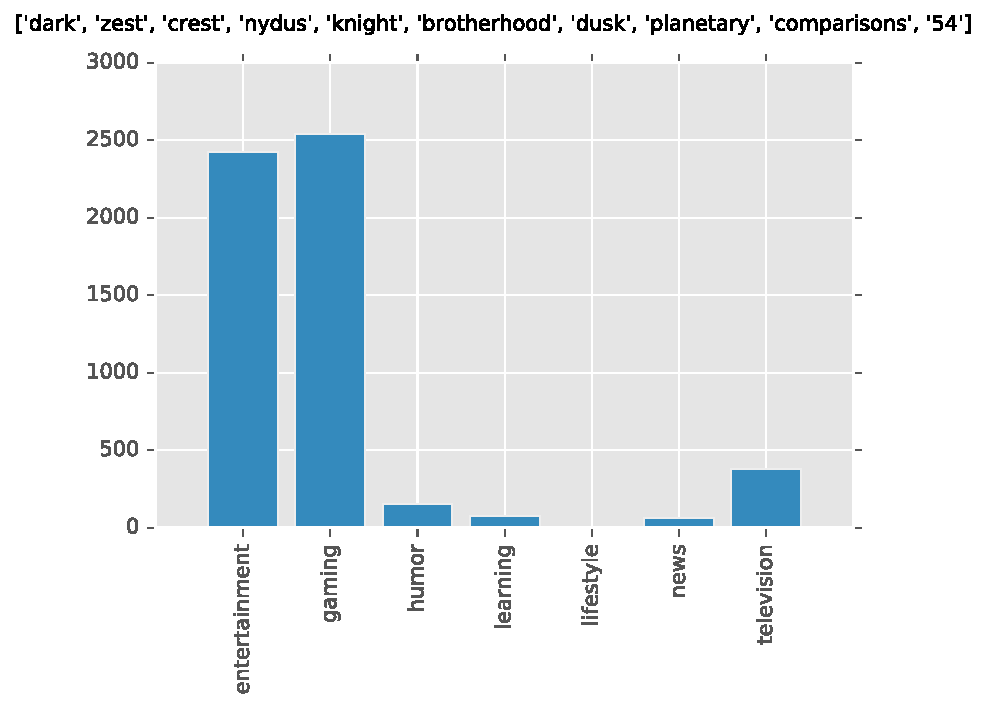
\includegraphics[]{figures/reddit-dark-5.pdf}
\caption{``dark'' sense 6}
\label{fig-reddit-dark-5}
\end{subfigure}
\begin{subfigure}[t]{.3\textwidth}
\centering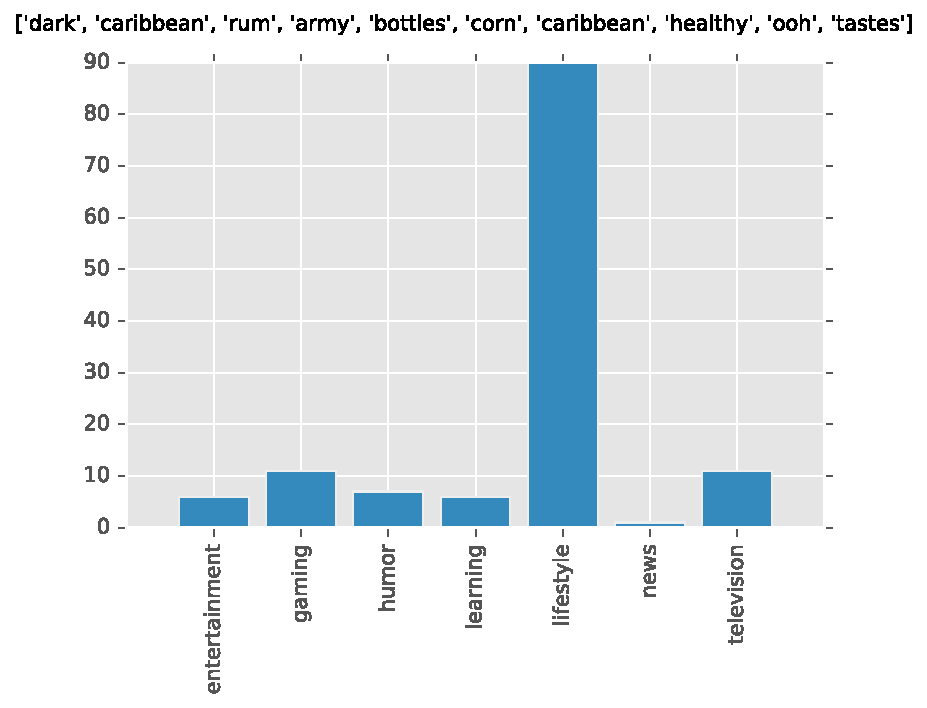
\includegraphics[]{figures/reddit-dark-6.pdf}
\caption{``dark'' sense 1}
\label{fig-reddit-dark-7}
\end{subfigure}
\caption{The different senses of the word ``dark'' together with the words most similar to the particular sense of ``dark''.}
\label{fig-reddit-dark} 
\end{figure}

\begin{figure}[H]
\begin{subfigure}[t]{.3\textwidth}
\centering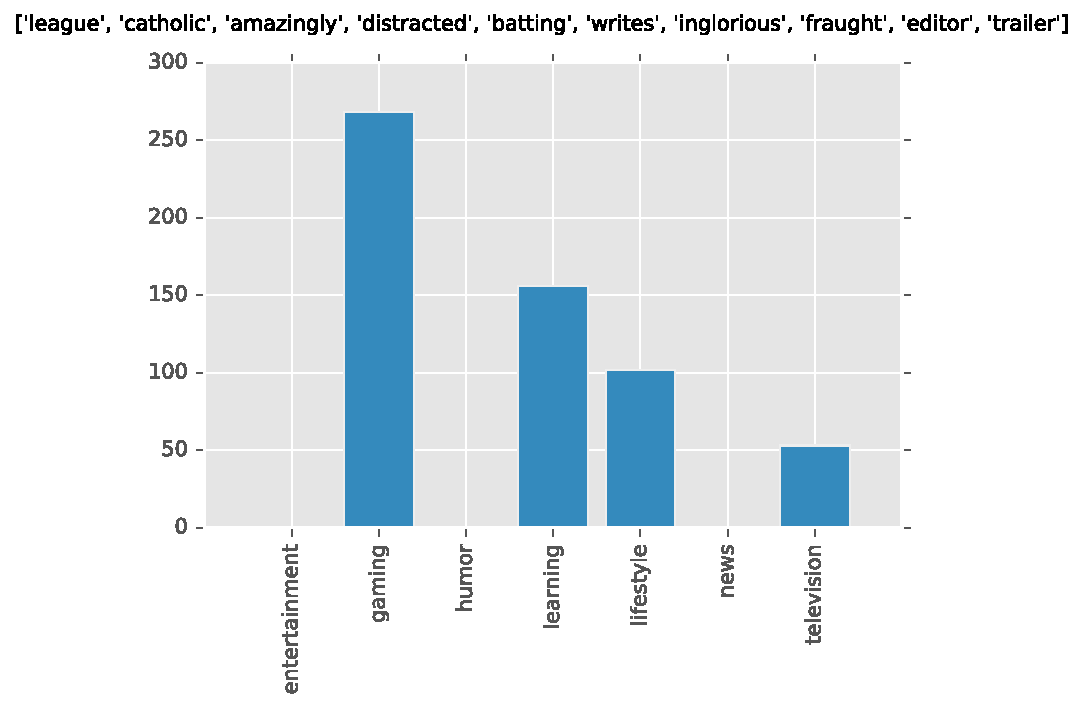
\includegraphics[]{figures/reddit-league-0.pdf}
\caption{``league'' sense 1}
\label{fig-reddit-league-0}
\end{subfigure}
\begin{subfigure}[t]{.3\textwidth}
\centering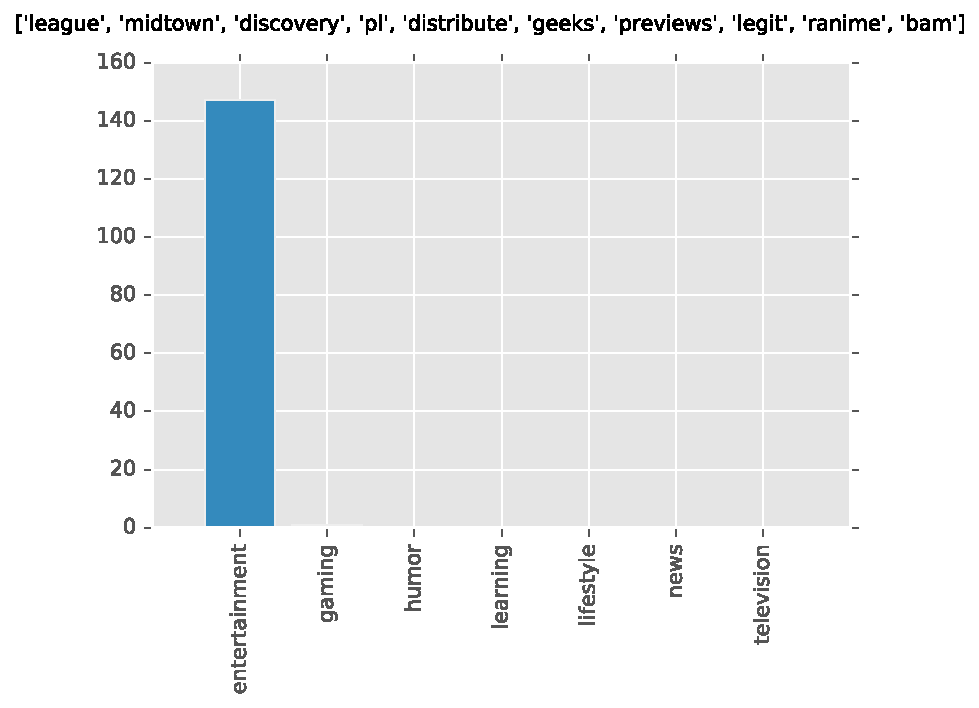
\includegraphics[]{figures/reddit-league-1.pdf}
\caption{``league'' sense 2}
\label{fig-reddit-league-1}
\end{subfigure}
\begin{subfigure}[t]{.3\textwidth}
\centering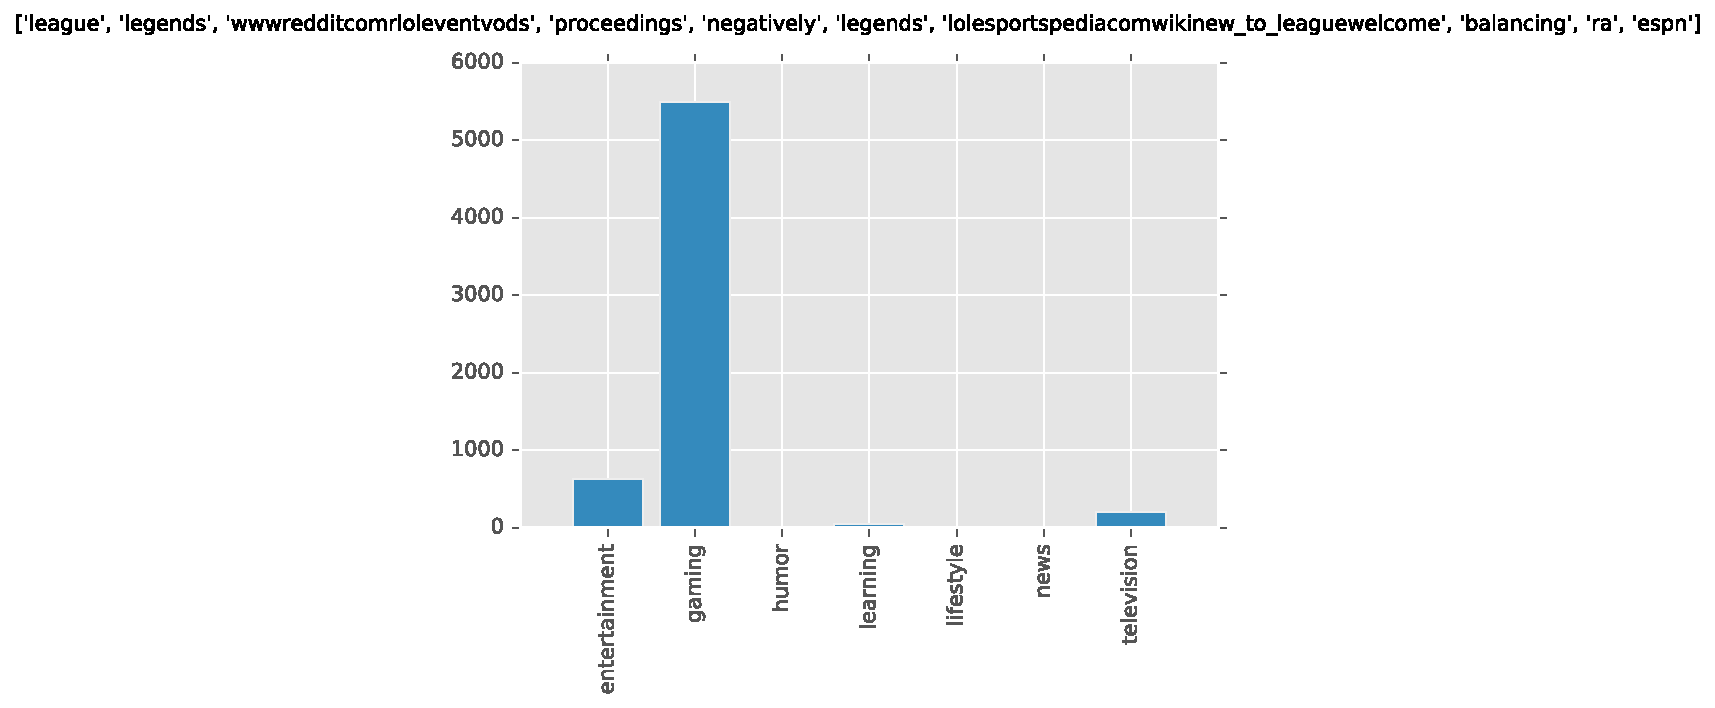
\includegraphics[]{figures/reddit-league-2.pdf}
\caption{``league'' sense 3}
\label{fig-reddit-league-2}
\end{subfigure}
\begin{subfigure}[t]{.3\textwidth}
\centering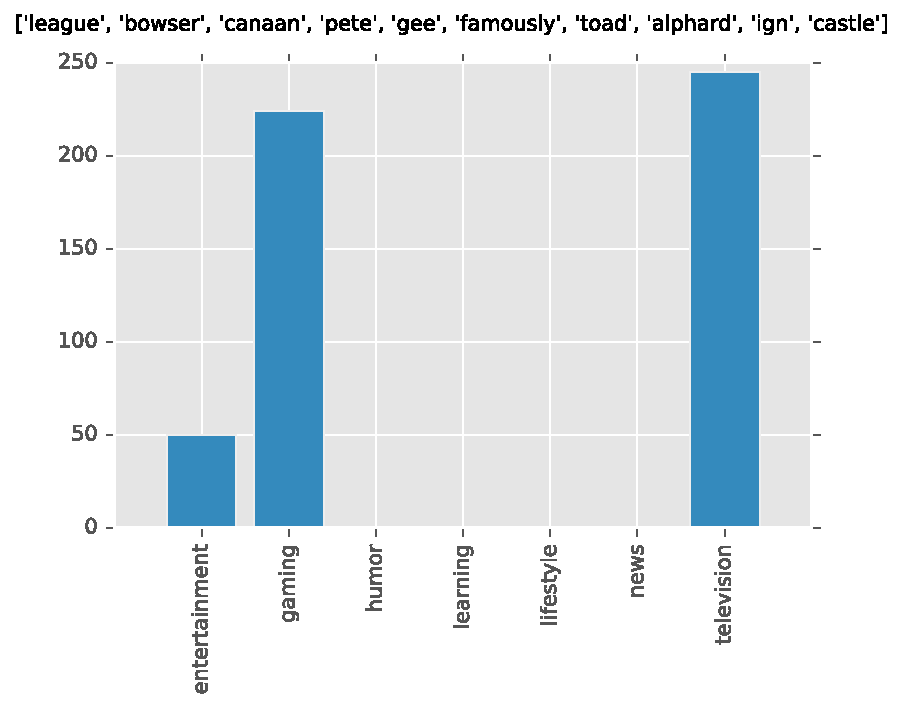
\includegraphics[]{figures/reddit-league-3.pdf}
\caption{``league'' sense 4}
\label{fig-reddit-league-3}
\end{subfigure}
\begin{subfigure}[t]{.3\textwidth}
\centering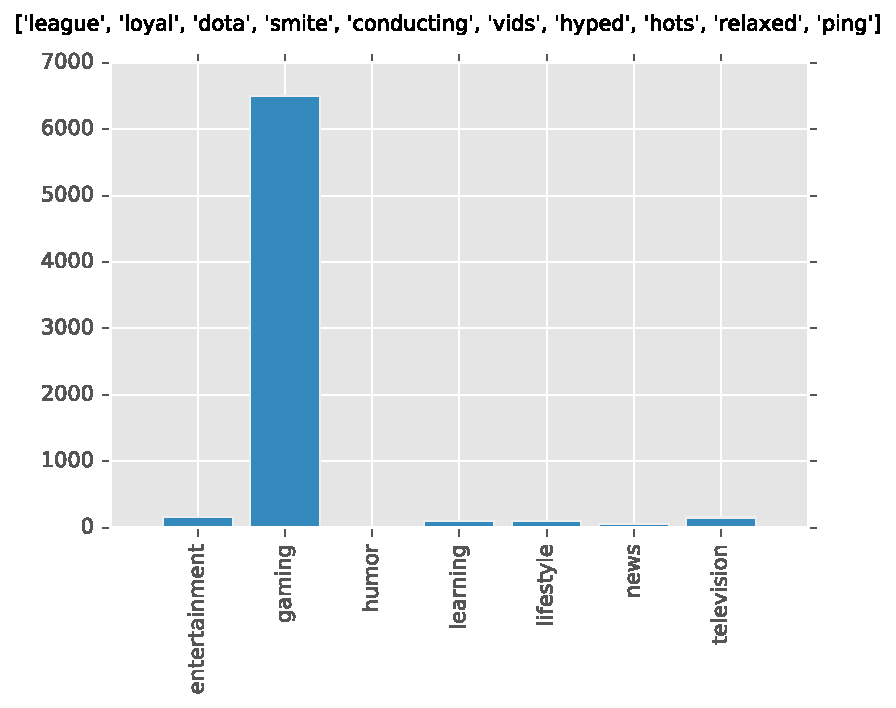
\includegraphics[]{figures/reddit-league-4.pdf}
\caption{``league'' sense 5}
\label{fig-reddit-league-4}
\end{subfigure}
\begin{subfigure}[t]{.3\textwidth}
\centering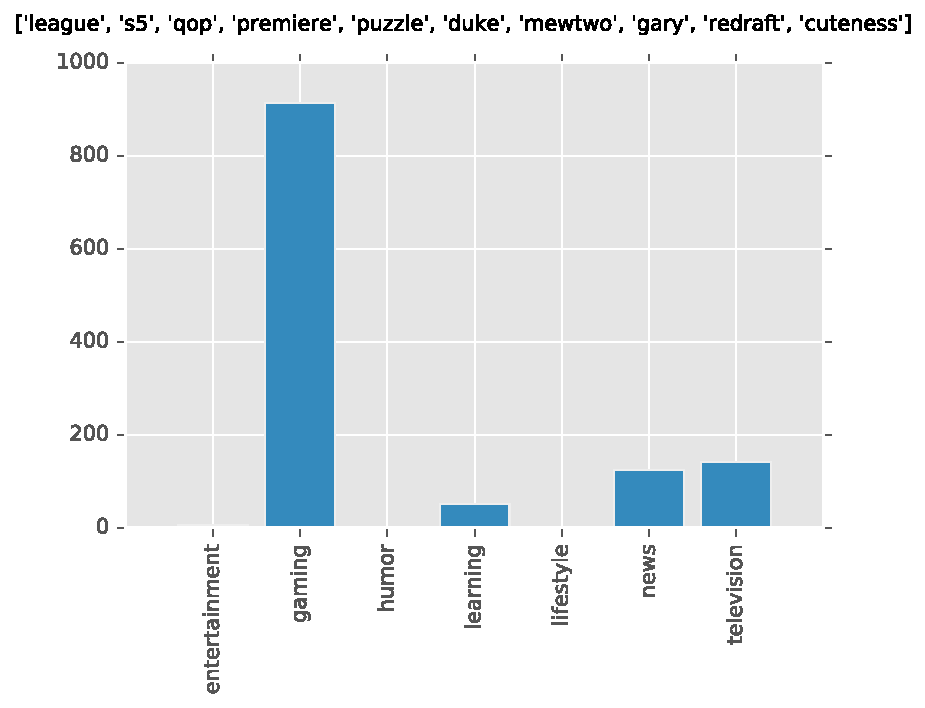
\includegraphics[]{figures/reddit-league-5.pdf}
\caption{``league'' sense 6}
\label{fig-reddit-league-5}
\end{subfigure}
\begin{subfigure}[t]{.3\textwidth}
\centering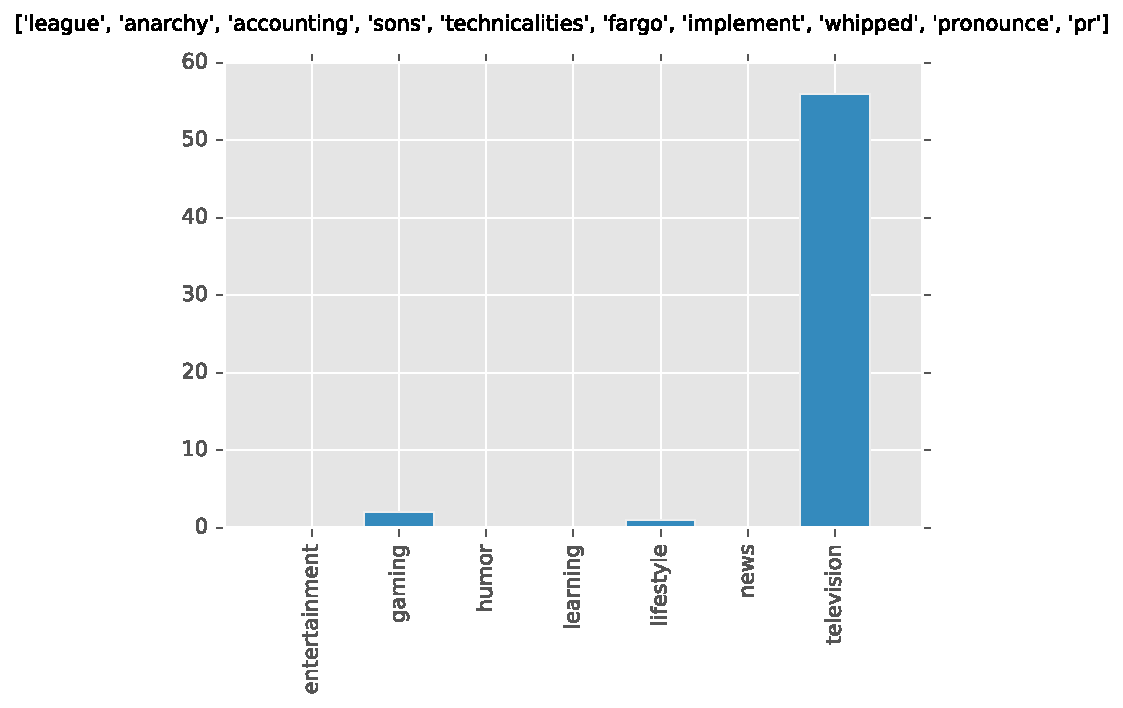
\includegraphics[]{figures/reddit-league-6.pdf}
\caption{``league'' sense 1}
\label{fig-reddit-league-7}
\end{subfigure}
\caption{The different senses of the word ``league'' together with the words most similar to the particular sense of ``league''.}
\label{fig-reddit-league} 
\end{figure}

\end{landscape}

\subsection{Identifying Community Word Usage using the MSSG Algorithm}

I test this histogram output on the reference Reddit corpus to see how users in different communities of Reddit use certain words.

Figure \ref{fig-reddit-dark-1} shows a ``dark'' being used in the context of science as in dark matter and dark energy. This sense appears predominantly in the \emph{learning} community which makes sense since this is the community that concerns itself with such topics. Figure \ref{fig-reddit-dark-2} shows ``dark'' being used in the context of the film / story Harry Potter as in dark wizards and dark lord. This predominantly appears in \emph{entertainment} and minorly so in \emph{television}, which again corresponds to intuition. Figure \ref{fig-reddit-dark-4} shows ``dark'' being used in the context of Pokemons as in ``dark Pokemons'', which is used predominantly in the \emph{gaming} community. Finally, and rather unexpectedly, ``dark'' is also used in the context of rum where it is used to describe dark rum. This is used predominantly in the \emph{lifestyle} community in the Reddit corpus.

It was similarly able to distinguish between ``league'' as used in sports and ``league'' as used in gaming (as in League of Legends) as shown in Figure \ref{fig-reddit-league}.

My algorithm adds on to \cite{neelakantan2015efficient} by allowing users to trace the source of the senses of words. This has the following applications:

\begin{itemize}
\item In codeword detection, I am now able to detect when different communities of people use a word different from the rest of their peers
\item In an organization, this can also be used to detect departments / groups of individuals that use a word (may not be a codeword) differently. For example, the name of a boss may be used pejoratively in one department and agreeably in another.
\end{itemize}

However, I still needed a method to systemize the detection of codewords from these histograms.

\subsection{Using KL Divergence to Systematically Identify Codewords}

I then used KL divergence to compare each histogram (for each sense of each word in the corpus) against the uniform distribution. The hypothesis is that a word (such as ``hello'') that is disambiguously used by everyone in the organization should have roughly equal chance of occurring in any of the communities (barring especially lopsided sizes of communities within the corpus, such as one single community taking up 90\% of the corpus). Hence, the sense of ``hello'' as in a greeting should have a near uniform distribution as shown in the ``apple'' example earlier.

The result of doing this is positive. The table below lists the KL divergences of each of the senses of the words in the first row in Figure \ref{fig-reddit-kl}.

\begin{table}[H]
\centering
\begin{tabular}{c c c c c}
\toprule
 good & money & people & dark & league \\
\midrule
0.14463918 & 0.00648365 & 0.16257816 & 0.22922427 & 0.71126526 \\
0.52091641 & 0.43071434 & 0.14932918 & 1.62014716 & 1.90541132 \\
0.06240066 & 0.44830668 & 0.20445455 & 1.59789641 & 1.42980752 \\
0.53456988 & 0.24518687 & 0.09279462 & 0.34249047 & 1.00348243 \\
0.07151459 & 0.14681329 & 0.05849862 & 1.54230648 & 1.54250742 \\
0.44972733 & 0.31814621 & 0.7711894 & 0.83141833 & 1.09152749 \\
0.54374559 & 0.74424692 & 0.1302974 & 0.79688892 & 1.71254201 \\
\bottomrule
\end{tabular}
\caption{KL divergence for each of the senses of the words. Words with rather uniform usage (``good'', ``money'', ``people'') have low KL divergences from the uniform distribution for all senses. However, the usages of ``dark'' and ``league'' highlighted earlier all have high KL divergences}
\label{fig-reddit-kl}
\end{table}

Then, selecting codewords would be a matter of selecting a threshold KL divergence.

\begin{figure}[h]
\centering
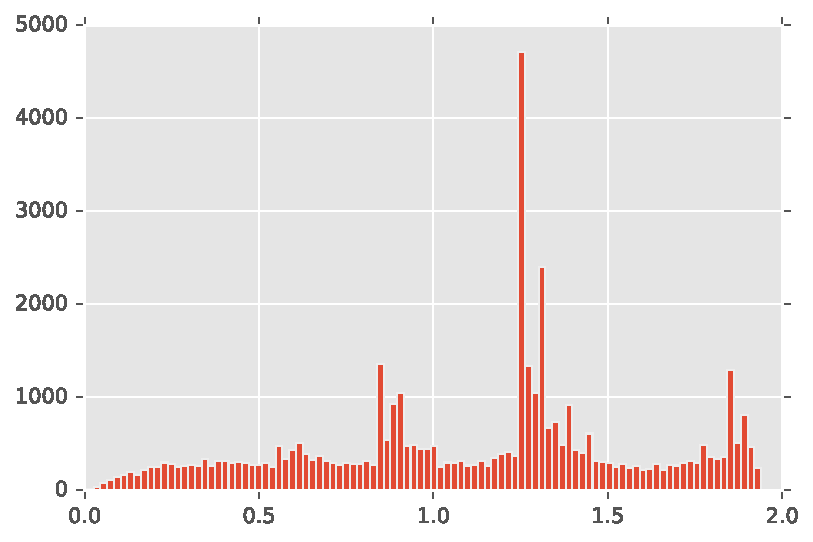
\includegraphics[width=.5\textwidth]{figures/reddit-community-histo.pdf}
\caption{KL divergence histogram for all words in the reddit corpus. Finding words that are used specially in a community would be to select a threshold KL divergence}
\label{fig-wsj-count}
\end{figure}

Unfortunately, I did not have time to follow through this.
